%%%%
% Преамбула: подключение необходимых пакетов
% Редактируйте осторожно!
%

\documentclass[hyperref={unicode}]{beamer}

\usepackage[utf8x]{inputenc}
\usepackage[english, russian]{babel}
\usepackage{color, colortbl}
\usepackage{rotating} 
\usepackage{graphicx}
\usepackage{algorithmic}

\usetheme[nosecheader]{PetrSU-CS}


%%%%
% Преамбула: основные параметры презентации
% Отредактируйте в соответствии с комментариями
%

\title[%
    % Краткое название работы не используется в этой презентации!
    % Бобры и Интернет
]{%
    % Полное название работы отображается на титульной странице
    Приложение <<Remote Control>>
}

% Подзаголовком опишите тип работы:
% - Курсовая работа
% - Выпускная квалификационная работа бакалавра
% - Дипломная работа
% - Магистерская диссертация
\subtitle{Отчет о проектной работе по курсу <<Разработка приложений для мобильных ОС>>}

\author[%
    % Имя и фамилия автора работы отображаются на каждом слайде в нижнем колонтитуле
    Татьяна Квист
]{%
    % Имя, отчество и фамилия автора работы отображаются на титульном слайде
    Татьяна Денисовна Квист
}

\date[%
    % Дата защиты
    28.05.2021
]{%
    % Руководитель
    Научный руководитель: ст. преп., А. В. Бородин
}

\institute[%
    % Краткое название организации не используется в этой презентации
    ПетрГУ
]{%
    % Полное название организации и подразделения
    Петрозаводский государственный университет\\
    Кафедра информатики и математического обеспечения
}


%%%%
%
% Начало содержимого слайдов
%

\begin{document}

% Титульный слайд
\begin{frame}
\maketitle
\end{frame}

% Пример слайда для обоснования актуальности работы
\begin{frame}
  % Заголовок слайда
  \frametitle{Проблема автоматизации}
  Всё больше и больше компаний создают предметы для умного дома. С помощью телефона можно настроить холоднильник, чайник и кофемашину. Но не стоит забывать и про интерьер, ведь от него многое зависит: как ваши гости оценят обстановку, праздничное настроение, да и настроение в целом. Одним из популярных укаршений является гирлянда. Поэтому предлагается создать пульт дистанционного управления для светодиодной ленты. 
\end{frame}

% Пример слайда с формулировкой целей и задач
\begin{frame}
  % Заголовок слайда
  \frametitle{Цель и задачи}
  \begin{block}{Цель работы}
    Разработать мобильное приложение для дистанционного управления светодиодной лентой.
  \end{block}
  \begin{block}{Задачи}
  \begin{itemize}
    \item Разработать модуль главной страницы;
    \item Разработать модуль для выбора монотонной подсветки;
    \item Разработать модуль для создания цветовой последовательности;
    \item Разработать модуль для выбора режима;
    \item Разработать модуль для создания градиента;
    \item Реализовать мобильное приложение с использованием разработанных модулей с использованием React Native и Expo.
  \end{itemize}
  \end{block}
\end{frame}

\begin{frame}
    % Заголовок слайда
    \frametitle{Этапы разработки приложения}
    \begin{enumerate}
        \item Разработка модуль главной страницы;
        \item Разработка модуль для выбора монотонной подсветки;
        \item Разработка модуль для создания цветовой последовательности;
        \item Разработка модуль для выбора режима;
        \item Разработка модуль для создания градиента;
    \end{enumerate}
\end{frame}
  
\begin{frame}
    % Заголовок слайда
    \frametitle{App.js}
    App.js --- основной модуль, содержащий в себе остальные модули интерфейса.
\end{frame}

\begin{frame}
    % Заголовок слайда
    \frametitle{MonoColor.js}
    MonoColor.js --- модуль с выбором цвета монотонной подсветки. Состоит из нескольких других модулей:
    \begin{itemize}
        \item ColorPalette.js --- модуль для отображения группы цветов.
        \item Color.js --- модуль для отображения цвета. Круг с диаметром в 25 пикселей. В качестве аргумента получает строку с цветом (hex, rgb или название). 
    \end{itemize}
\end{frame}

\begin{frame}
    % Заголовок слайда
    \frametitle{Sequence.js}
    Sequence.js --- модуль с выбором цветовой последовательности. Используются элементы, которые отвечают за выбор пользователя (три круга), которые меняются в зависимости от выбора. Состоит из нескольких других модулей:
    \begin{itemize}
        \item ColorPaletteSmallSeq.js --- модуль для отображения группы цветов.
        \item ColorSmall.js --- модуль для отображения цвета. Круг с диаметром в 20 пикселей. В качестве аргумента получает строку с цветом (hex, rgb или название). 
    \end{itemize}
\end{frame}

\begin{frame}
    \frametitle{Modes.js}

    Modes.js --- модуль с выбором режима подсветки. Всего есть два режима: радуга (на каждом светодиоде одинаковый цвет в один момент времени) и горизонтальная радуга (на каждом светодиоде разный цвет в один момент времени).
\end{frame}

\begin{frame}
    \frametitle{Gradient.js}

    Gradient.js --- модуль с выбором градиента. Пользователь выбирает два цвета, из которых создаётся линейный градиент. Состоит из нескольких других модулей:
    \begin{itemize}
        \item ColorPaletteSmallGrad.js --- модуль для отображения группы цветов.
        \item ColorSmall.js 
    \end{itemize}
\end{frame}

% Пример заключительного слайда
\begin{frame}
  \frametitle{Заключение}
  
  Реализованно:
  
  \begin{itemize}
    \item Корректное отображение всех элементов;
    \item Отображение выбора пользователя;
    \item Отправка данных на сервер.
  \end{itemize}
  
\end{frame}

\begin{frame}
    \frametitle{Заключение}
    
    В результате проекта было разработано мобильное приложение для дистанционного управления светодиодной лентой. Пользователь может выбрать монотонное освещение, последовательность цветов, уже запрограммированный режим или выбрать два цвета для линейного градиента.\\

\end{frame}

\begin{frame}
    \centering
    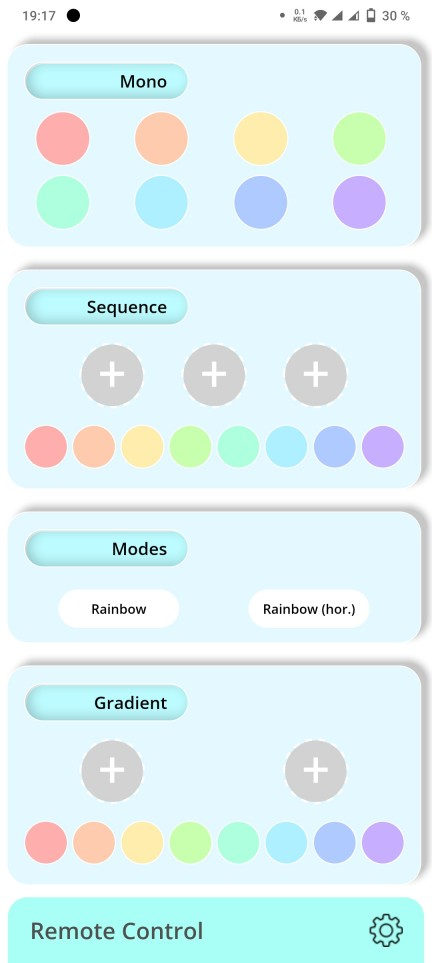
\includegraphics[width = .3\textwidth]{app.jpg}
\end{frame}

\begin{frame}
    \frametitle{Заключение}
    Предлагаемые дополнения для реализации: 
    \begin{itemize}
        \item изменение темы приложения (ночной режим);
        \item возможность добавлять свои цвета.
    \end{itemize}
    
\end{frame}
  
% \begin{frame}
%   \frametitle{}
  
% {\Large\mbox{}\hfil Спасибо за внимание!}
  
% \end{frame}
\end{document}
